\chapter{Модель самоструктурирующихся сообществ Ульфа Дикмана}

В данной части настоящей работы вводится модель самоструктурирующихся в пространстве сообществ, предложенная Ульфом Дикманом (Ulf Dieckmann)  и Ричардом Лоу (Richard Law) в \cite{law_dieckmann_2000,law_2003}; вводится предлагаемое пространство состояний системы, описываемой набором статистик, отвечающих за естественные степени свободы популяции; описывается пространство параметров системы и динамика предложенный статистик относительно данного пространства параметров; обсуждается техника аппроксимаций (замыканий) набора статистик высшего порядка при помощи статистик младших порядков.

Отдельно необходимо отметить, что предлагаемое описание модели основано на работе \cite{law_dieckmann_2000} и не ставит перед собой цель формального построения всех используемых выкладок; вопрос формализации используемой модели обсуждался в \cite{egor}, где было показано, что подобная формализация может быть выполнена без потери корректности итоговых интегро-дифференциальных уравнений динамики.

\section{Пространственные моменты как набор статистик для описания популяции}

Положим, что рассматриваемая популяция заселяет некоторую конечную область пространства, которую будем обозначать $A \subset \mathbb{R}^d$, где $d = 1, 2, 3$; соответственно объем (или меру)  данной области, в общем его понимании, будем обозначать $|A|$. Также допустим, что число различных видов в популяции конечно и равно $n$; для удобства пронумеруем сами виды и далее будем обращаться к ним только по нумерации. Также положим $X^i_t$ --- множество точек, в которых присутствует индивид $i$-го вида в момент времени $t$ (в рамках нашей модели договоримся считать особи безразмерными; вопрос о моделировании размера особи может быть решен в рамках нашей модели, как будет указано позже).

\textbf{Определение 1.} Паттерном $p(x)$ будем называть следующую вектор-функцию
\begin{equation*}
p(x)=\left(p_{1}(x),\;p_{2}(x),\ldots,\:p_{n}(x)\right), 
\end{equation*}
где $ p_{i}(x) $ --- паттерн $ i- $го вида, равный
\begin{equation*}
p_{i}(x)=\sum_{x'\in X_t^i}\delta(x-x'),
\end{equation*}
где $ \delta(x) $ --- дельта-функция Дирака. Как следует из определения паттерна, он описывает распределение особей и структуру всего сообщества в \textit{конкретный момент времени}. Поэтому зависимость некоторой величины от паттерна стоит понимать как "при конкретном распределении". Более того, ясно если рассмотреть пространство всех паттернов, то в зависимости  от параметров системы тот или иной паттерн более вероятен в определенный момент времени, т.е. на пространстве паттернов можно задать вероятностную меру, зависящую от времени (формализация подобного подхода описана в \cite{egor}).

Пользуясь известным свойством функции Дирака, не составляет труда выразить среднюю плотность индивидов $ i- $го вида в области через пространственный паттерн:
\begin{equation*}
N_{i}(p)=\frac{1}{|A|}\int_{A}p_{i}(x)dx
\end{equation*}

\textbf{Определение 2.} Первым моментом (средней ожидаемой плотностью индивидов) $ i- $го вида будем называть математическое ожидание средних плотностей $N_{i}(p)$ в момент времени $t$ по всему пространству паттернов для фиксированного времени:
\begin{equation*}
N_{i}(t)=\mathbb{E}_{p}N_{i}(p)
\end{equation*}

Аналогично введем функцию, возвращающую число пар индивидов данных видов $ i $ и $ j $, находящихся на расстоянии $ \xi $ (функцию парной корреляции):
\begin{equation*}
\hat{C}_{ij}(\xi,p)=\frac{1}{|A|}\int_{A}p_{i}(x)[p_{j}(x+\xi)-\delta_{ij}\delta_{x}(x+\xi)]dx
\end{equation*}

\textbf{Определение 3.} Вторым пространственным моментов (средней ожидаемой плотностью пар) особей видов $ i $ и $ j $ таких, что $\vec{x}_j=\vec{x}_i+\vec{\xi}$, где $\vec{x}_i$, $\vec{x}_j$ --- расположение особей $i$-го и $j$-го вида соответственно, назовем математическое ожидание:
\begin{equation*}
C_{ij}(\xi,t)=\mathbb{E}_{p}\hat{C}_{ij}(\xi,p)
\end{equation*}

В рамках нашей модели будем считать, что все взаимодействия между индивидами мелкомасштабны. Таким образом, наличие пространственной структуры между достаточно удаленными особями не является существенным; более того, из этого следует, что особи, "унесенные" на бесконечность, теряют пространственную структуру, т.е. корреляционная функция вырождается до произведения средних плотностей:
\begin{equation*}
\lim_{|\xi|\to\infty}C_{ij}(\xi,t)=N_{i}(t)N_{j}(t)
\end{equation*}

Аналогично, можно доопределить плотность и более общих пространственных структур: 
\begin{equation*}
\hat{C}_{i_{1}\ldots i_{m}}(\xi_{1},\ldots,\xi_{m-1},p)=\frac{1}{|A|}\int_{A}p_{i}(x)\prod_{j=2}^{m}p_{j_{j}}(x+\xi_{j-1})dx
\end{equation*}
\begin{equation*}
C_{i_{1}\ldots i_{m}}(\xi_{1},\ldots,\xi_{m-1},t)=\mathbb{E}_{p}\hat{C}_{i_{1}\ldots i_{m}}(\xi_{1},\ldots,\xi_{m-1},p),
\end{equation*}
где вектора $\xi_{l}$ определяются аналогично парной корреляционной функции как вектор между расположением особи вида $i_1$ и $i_{l+1}$. В рамках нашего исследования существенное значение будут иметь только пространственные моменты третьего порядка $ T_{ijk}(\xi,\xi',t) $ --- плотности троек индивидов.

\textbf{Предложение 1.} Описанная система пространственных моментов, согласно исследуемой модели, есть набор статистик для описания естественных степеней свободы системы; более того, как будет показано далее, для исследования пространственной структуры мы будем ограничиваться первыми двумя моментами и аппроксимацией на корреляционную функцию троек.

\section{События динамики модели}

Как было указано выше, рассматриваемая модель опирается на описание событий для каждого индивида популяции, причем события допустимы трех следующих видов --- рождение нового индивида, гибель индивида и перемещение индивида в геометрическом пространстве.

В рамках нашего исследования ограничимся стационарными моделями, т.е. сообществами, в которых движение реализовано исключительно за счет рождения новой особи; например, будем считать, что рассматриваются только растительные сообщества. Данная договоренность введена в целях упрощения выявления существенных эффектов пространственной неоднородности, что было бы сложнее сделать в сильно диффузируюищх популяциях.

\subsection{Рождение нового индивида}

Вероятность рождения потомка вида $i$, которая будет зависеть от расстояния, на котором рождается потомок, в точке $ \xi' $ от родителя, находящегося в точке $ \xi $ будем обозначать
\begin{equation*}
B_{i}(\xi,\xi')=m_{i}(\xi'-\xi),
\end{equation*}
где функцию $ m_{i}(x) $ есть ядро рождения (ядро распространения, dispersal kernel). $ \int_{\mathbb{R}^{n}}m_{i}(x)dx=b_{i} $ --- темп рождаемости, $ 0<b_{i}<1 $, привычная константа, описывающая темп рождаемости в логистической модели. 

В данной работе будем считать, что $ \frac{1}{b_{i}}m_{i}(x) $ распределено нормально с нулевым матожиданием $ \left(m_{i}\sim N(0,\sigma_{i}^{m})\right) $; также положим $ m_{i} $ радиально-симметричной ($ m_{i}(x)=m_{i}(|x|) $) из биологических соображений. В то же время следует отметить, выбор нормального распределения, обусловленный центральной предельной теоремой, не является единственным подходящим; в целях моделирования ненулевого размера индивида ядра распространения может быть выбрано с плато в окрестности 0:
\begin{equation*}
m(\xi)=\hat{b}_m \xi^4 \cdot e^\frac{-\xi^2}{1+\sigma^2_m\xi^4}
\end{equation*}


\subsection{Гибель индивида}

Вероятность гибель конкретного индивида в данной точке $\xi$ очевидным образом определяется не только влиянием среды (параметр логистической модели), но также и расположением всех остальных индивидов в популяции, причем не только их количеством, но и пространственной структурой:
\begin{equation*}
D_{i}(\xi,p)=d_{i}+\sum_{j}\int_{\mathbb{R}^{n}}w_{ij}\left(\xi-\xi'\right)\left[p_{j}(\xi')-\delta_{ij}\delta_{x}(\xi')\right]d\xi',
\end{equation*}
где $ d_{i} $ --- экзогенная вероятность смерти, т.е. смерти от влияния окружающей среды (полагаем его пространственно постоянным; несложно заметить, что введения некого пространственного градиента у данной величины существенной не усложнит модель и получающиеся уравнения), $ 0<d_{i}<1 $; $ w_{ij}(x) $ --- ядро конкуренции (competition kernel) --- плотность вероятности смерти индивида $ i- $го вида от конкуренции с индивидом $ j- $го вида, находящимся на расстоянии $ x $, $ \int_{\mathbb{R}^{n}}w_{ij}(x)dx=d'_{ij} $ --- агрегированная сила конкуренции, $ 0<d'_{ij}<1 $. 

В данной работе будем считать, что $ \frac{1}{d'_{ij}}w_{ij}(x) $ распределено нормально с нулевым математическим ожиданием $ \left(w_{ij}\sim N(0,\sigma_{ij}^{w})\right) $; также положим $ w_{ij} $ радиально-симметричной ($ w_{ij}(x)=w_{ij}(|x|) $) из биологических соображений. Здесь также можно отметить, что биологически более разумным возможно было бы использование ядра с сингулярностью вокруг 0.

\section{Динамика пространственных моментов}

\textbf{Предложение 2. } Заметим, что переход из одного паттерна в другой есть цепочка описанных выше событий. Допустим теперь, что для данного паттерна $p_0$ мы посчитали плотность вероятности перехода во все остальные паттерны за время $\tau$. Устремляя теперь $\tau \to 0$, мы получаем с одной стороны производную плотности вероятности перехода, а с другой --- переход в паттерн, удаленный ровно на одно событие из описанных выше (из-за бескончно малого промежутка времени). Данное соображение позволяет в частности выписать уравнения динамики пространственных моментов.

Полный вывод данных уравнений приведен в \cite{law_dieckmann_2000}, мы же воспользуемся полученным результатом:
\begin{equation*}
\frac{d}{dt}N_{i}=(b_{i}-d_{i})N_{i}-\sum_{j}\int_{\mathbb{R}^{n}}w_{ij}(\xi)C_{ij}(\xi)d\xi
\end{equation*}
Аналогично случаю логистической модели, каждое слагаемое в приведенной уравнении может быть проинтерпретированно с биологической точки зрения:
\begin{itemize}
\item $ b_{i}N_{i} $ --- математическое ожидание количества новых рожденных индивидов от всех родителей в популяции;

\item $ d_{i}N_{i} $ --- математическое ожидание количества смертей индивидов от воздействия окружающей среды;

\item $ \sum_{j}\int_{\mathbb{R}^{n}}w_{ij}(\xi)C_{ij}(\xi)d\xi $ --- математическое ожидание особей, умерших от конкуренции; функция парной корреляции здесь представляет ничто иное как \textit{весовую функцию конкуренции}.
\end{itemize}

Подобное уравнение динамики можно составить и для парной корреляции:
\begin{multline*}
\frac{d}{dt}C_{ij}(\xi)	=	\delta_{ij}m_{i}(-\xi)N_{i}+\int_{\mathbb{\mathbb{R}}^{n}}m_{i}(\xi')C_{ij}(\xi+\xi')d\xi'-d_{i}C_{ij}(\xi)-\\
-\sum_{k}\int_{\mathbb{\mathbb{R}}^{n}}w_{ik}(\xi')T_{ijk}(\xi,\xi')d\xi-w_{ij}(\xi)C_{ij}(\xi)+\langle i,j,\xi\to j,i,-\xi\rangle,
\end{multline*}
где слагаемое $ \langle i,j,\xi\to j,i,-\xi\rangle $ следует читать как повторение всех предыдущих членов с точностью до описанной замены; это объясняется тем, что ранее  мы рассматривали вероятности исключительно для особи $i$-го вида в паре.

Здесь так же можно охарактеризовать каждое слагаемое:
\begin{itemize}
	\item $ \delta_{ij}m_{i}(-\xi)N_{i} $ --- если мы рассматриваем случай  интравидовой корреляции, то новая пара может возникнуть, если от потомка до родителя будет вектор $-\xi$ (ясно, что в случае $i \ne j$ нужны исключительно пары с положительным знаком);
	
	\item  $ \int_{\mathbb{\mathbb{R}}^{n}}m_{i}(\xi')C_{ij}(\xi+\xi')d\xi' $ --- искомая пара возникает, если первая особь в паре (вида $i$) создаст потомка таким образом, что потомок и вторая особь в паре окажутся на расстоянии $\xi$;
	
	\item $ d_{i}C_{ij}(\xi) $ --- пара может быть разрушена из-за экзогенной смерти особи $i$-го вида в паре;
	
	\item $ w_{ij}(\xi)C_{ij}(\xi) $ --- также пара может быть разрушена в следствие конкуренции внутри пары (данное слагаемое приходится учитывать, поскольку из-за задания пространственных моментов через дельта функции все пространственный структуры приняты в общем положении);
	
	\item  $ \sum_{k}\int_{\mathbb{\mathbb{R}}^{n}}w_{ik}(\xi')T_{ijk}(\xi,\xi')d\xi-w_{ij}(\xi)C_{ij}(\xi) $ --- также существует вероятность смерти особи вида $i$ из-за конкуренции с остальными особями в популяции, т.е. весовая функция такой конкуренции --- это структура троек $ T_{ijk} $ с одним фиксированным расстоянием  $\xi$.
\end{itemize}

\section{Замыкания пространственных моментов}

\textbf{Замечание 1.} Приведенный биологический смысл динамики пространственных моментов позволяет сделать следующее наблюдение: динамика пространственного момента всегда должна включать слагаемое, отвечающее за гибель одной из особей этой пространственной структуры вследствие конкуренции с оставшимися особями в популяции. Весовая функция данной конкуренции есть пространственный момент более высокого порядка, поскольку это и есть плотность более сложной пространственной структуры.

В результате динамика пространственного момента $k$-го порядка зависит от пространственного момента $k+1$-го порядка, что порождает счетную иерархию зависимостей и делает невозможным численный и аналитический анализ системы. Для сведения получающейся счетной системы интегро-дифференциальных уравнений к конечной системе используется техника замыканий, широко применяемая в статистической физике и физике плазмы.

\textbf{Определение 4.} Замыканием (аппроксимацией) пространственных моментов называется выражение момента порядка $k$ через моменты строго меньшего порядка.

\textbf{Предложение 3.} В \cite{law_dieckmann_2000,murlaw} было предложено исключить из рассмотрения замыкания моментов страше третьего порядка; моменты же третьего порядка следует замыкать через моменты первого и второго порядка, $ T_{ijk}=F(C_{ab},N_{c}) $, где $a, b, c \in \{i, j , k\}$. По предположению, выдвинутому в данных работах, эффекты моментов высших порядков на итоговую численность сообщества и его пространственную структуры пренебрежимо малы; корректность данного предположения будет обсуждаться ниже.

Дополнительным интересным аспектом изучаемой модели является то, что исследование замыканий моментов второго порядка, например
\begin{equation*}
C_{ij}(\xi,t)=N_{i}(t)N_{j}(t)
\end{equation*}
\begin{equation*}
C_{ij}(\xi,t)=N_{i}(t)N_{j}(t)(1+\varphi(\xi))
\end{equation*}
приводят в первом случае к логистической модели, а во втором --- к обобщенной логистической модели Лотки-Вольтерры, которая не является качественным инструментом для изучения самоструктурирующихся в пространстве сообществ, как уже обсуждалось во введении к данной работе.

\subsection{Требования на замыкания}

Введенное определение не накладывает никаких ограничений на функцию $F(C_{ab}, N_c)$ ($ T_{ijk}=F(C_{ab},N_c) $, где $a, b, c \in \{i, j , k\}$); однако ясно, что существует набор требований, которые должны выполняться, из-за биологического смысла величины $T_{ijk}$ как плотности троек индивидов. 

Более подробно данный вопрос освещен в \cite{murlaw}; здесь же мы опишем некоторые базовые ограничения, базовая идея которых заключается в том, что условие отсутствия пространственной структуры для больших расстояний должно сохраняться:
\begin{enumerate}
	\item $  T_{ijk}(\xi,\xi')\ge0 $ --- плотность всегда неотрицательна;
	
	\item $ T_{ijk}(\xi,\xi')=T_{jik}(-\xi,\xi'-\xi)=T_{kij}(-\xi',\xi-\xi') $ --- исходя из определения, $\xi$ и $\xi'$ --- это вектора конкретно между $i$--$j$-ой и $i$--$k$-ой особью; поэтому перестановка вершин должна влиять на векторные аргументы;
	
	\item если $C_{ij}=N_{i}N_{j} $, то $ T_{ijk}=N_{i}N_{j}N_{k} $, т.е. отсутствие пространственной структуры на более низком уровне должно запрещать ее и на более высоком;
	
	\item $ \lim_{\xi\to\infty}T_{ijk}(\xi,\xi')=N_{i}C_{jk}(\xi'-\xi) $ --- благодаря меломасштабности, унесенная на бесконечность точка разрушает пространственную структуру (в то же время она остается между двумя нетронутыми); аналогично $\lim_{\xi'\to\infty}T_{ijk}(\xi,\xi')=C_{ij}(\xi)N_{k} $;
	
	\item $  \frac{1}{|A|}\int_{\mathbb{R}^{n}}T_{ijk}(\xi,\xi')d\xi'=C_{ij}(\xi)N_{k} $ --- суммарное количество троек есть количество пар на плотность оставшегося вида.
\end{enumerate}


\subsection{Достаточное требование на замыкания}

Приведенные ограничения не позволяют установить качество выбранного замыкания, а только указывают на то, может ли в принципе выбранная функция являться им. Для проверки корректности замыкания (аппроксимации) используется техника сравнения результатов работы динамики модели (посчитанная при помощи классического метода решения дифференциальных уравнений Рунге-Кутты) с результатами работы individual-based стохастических компьютерных симуляций.

С результатами вычислений в \cite{law_dieckmann_2000} сравнивалось несколько кандидатов:
\begin{align*}
(1) \qquad & T_{ijk}(\xi,\xi')\approx C_{ij}(\xi)N_{k}+C_{ik}(\xi')N_{j}+C_{jk}(\xi-\xi')N_{i}-2N_{i}N_{j}N_{k};\\
(2) \qquad &  T_{ijk}(\xi,\xi')\approx\frac{1}{2}\left[\frac{C_{ij}(\xi)C_{ik}(\xi')}{N_{i}}+\frac{C_{ij}(\xi)C_{jk}(\xi'-\xi)}{N_{j}}+\frac{C_{ik}(\xi')C_{jk}(\xi'-\xi)}{N_{k}}-N_{i}N_{j}N_{k}\right];
\\
(3) \qquad & T_{ijk}(\xi,\xi')\approx\frac{C_{ij}(\xi)C_{ik}(\xi')}{N_{i}};
\\
(4) \qquad &    T_{ijk}(\xi,\xi')\approx\frac{C_{ij}(\xi)C_{ik}(\xi')C_{jk}(\xi'-\xi)}{N_{i}N_{j}N_{k}}.
\end{align*}

Результаты сравнения корректности работы каждого из кандидатов в замыкания представлены на рисунке \ref{fig:comp1}: в случае двухвидовой популяции производится сравнение фазовых портретов в фазовом пространстве $[N_1; N_2]$ (рис. \ref{fig:comp1:1}); для одновидовой популяции приведен график $N(t)$ (рис. \ref{fig:comp1:2}). Приведенные графики показывают наиболее подходящее из приведенных замыкание:
\begin{equation*}
T_{ijk}(\xi,\xi')\approx\frac{C_{ij}(\xi)C_{ik}(\xi')}{N_{i}}
\end{equation*}

Однако в работах автора \cite{as1, as2} было показано, что использование указанного замыкания в случае двухвидовой популяции приводит к одновидовым уравнениям, изученным в \cite{nik}, которые имеют решения только в случае $d=0$; для двухвидовой модели это означает $d'_{12}=d'_{21}$ и  $d_1=d_2$, т.е. отсутствует не только экзогенная смертность, но и межвидовая конкуренция, что биологически невозможно.

Предложенная в \cite{as2} квадратичная регуляризация интравидовых третьих моментов:
\begin{equation*}
T_{iii}(\xi,\xi')\approx\frac{1}{2}\left[\frac{C_{ii}(\xi)C_{ii}(\xi')}{N_{i}}+\frac{C_{ii}(\xi)C_{ii}(\xi'-\xi)}{N_{i}}+\frac{C_{ii}(\xi')C_{ii}(\xi'-\xi)}{N_{i}}-N^3_{i}\right]
\end{equation*}
приводит к системе, которая имеет нетривиальные решения. Однако эти решения напрямую противоречат найденным методами стохастических компьютерных симуляций механизмам сосуществования, предложенным в \cite{MURRELL}.

\begin{figure*}[ht]
	\centering
	\begin{subfigure}{.5\textwidth}
		\centering
		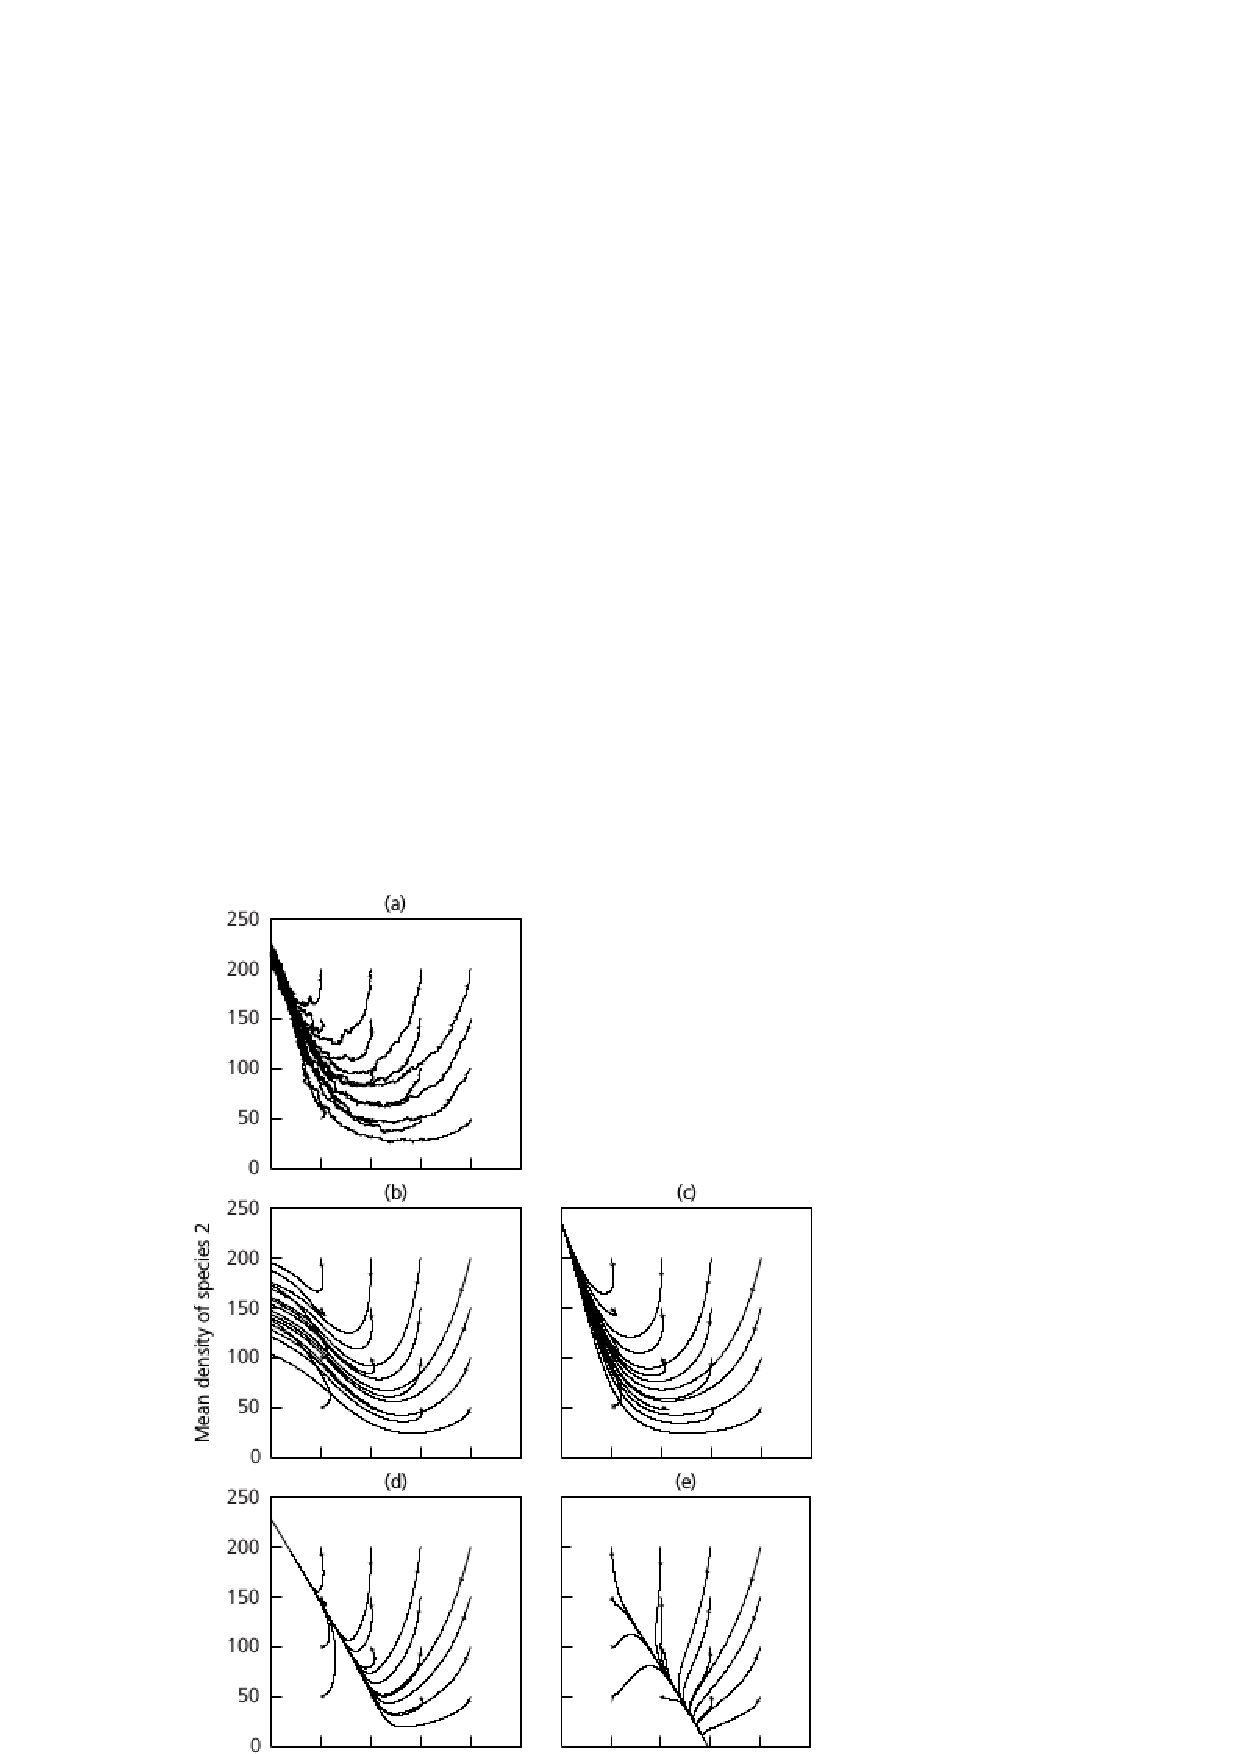
\includegraphics[width=.95\linewidth]{1234.png}
		\caption{Фазовый портрет в пространстве $[N_1; N_2]$: (a) --- для компьютерных симуляций; (b) -- (e) соответствуют решениям динамики по методы Рунге-Кутты для замыканий (1) -- (4) соответственно}
		\label{fig:comp1:1}
	\end{subfigure}% 
	\begin{subfigure}{.5\textwidth}
		\centering
		\includegraphics[width=.95\linewidth]{12345.jpg}
		\caption{Динамика первого момента $N(t)$ в случае одновидовой модели в сравнении с нескольким усредненными запусками симуляций} 
		\label{fig:comp1:2}
	\end{subfigure}
	\caption{Сравнение работы кандидатов в замыкания (1) -- (4) для одновидовых и двувидовых симуляций}
	\label{fig:comp1}
\end{figure*}

В то же время в \cite{murlaw} было предложено и исследовано параметрическое семейство замыканий:
\begin{multline}\label{eq:closure}
T_{ijk}(\xi,\xi')	=	\frac{\alpha}{2}\left(\frac{C_{ij}(\xi)C_{ik}(\xi')}{N_{i}}+\frac{C_{ij}(\xi)C_{jk}(\xi'-\xi)}{N_{j}}+\right.\\ 
\left.+\frac{C_{ik}(\xi')C_{jk}(\xi'-\xi)}{N_{k}}-1\right)+(1-\alpha)\frac{C_{ij}(\xi)C_{ik}(\xi')}{N_{i}},
\end{multline}
которое является линейной комбинацией замыканий (2) и (3). 
\begin{figure*}[ht]
	\centering
		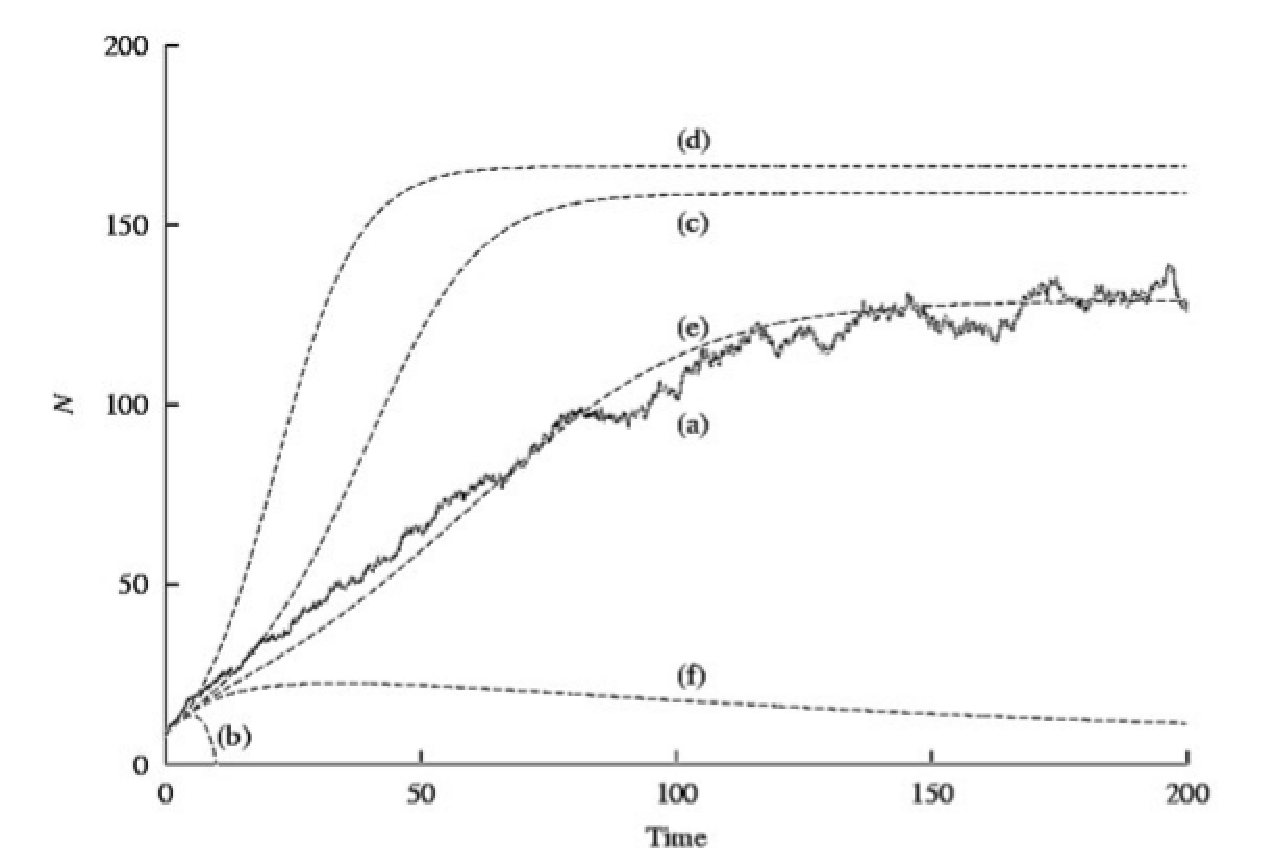
\includegraphics[width=.75\linewidth]{closures.eps}
		\caption{Сравнение работы различных представителей параметрического семейства замыканий с компьютерными симуляциями (a): (b) $\alpha = 1$; (c) $\alpha =0$; (d) $\alpha=1/4$; (e) $\alpha=2/5$}
	\label{fig:comp2}
\end{figure*}

Согласно результатам проверки на корректность различных представителей семейства предложенного замыкания в случае одновидовой системы, представленным на рис. \ref{fig:comp2}, наиболее подходящее под симуляции замыкание достигается при $\alpha = \frac{2}{5} $. Данное замыкание структурно достаточно близко к предложенной в \cite{as2} регуляризации, что приводит к совместной системе интегро-дифференциальных уравнений, в то время как предложенное замыкание работает более корректно; при всем этом стоит отдельно отметить, что используемое замыкание необязательно является наиболее подходящим и задача о поиске наиболее оптимального замыкания, не ограничиваясь выбранным семейством, является в известной мере одной из самых актуальных.